% BACKGROUND
% - What technology is the project based on?
%   - Describe the concept of the \ac{FREEDM} smart-grid
%   - Introduce the idea of using GM to coordinate power resources
%   - Introduce LB as the algorithm that acctually applies the transactions and migrates power
%       - Describe as a flow control algorithm
%   - RED/ECN as a network management technique
%       - \ac{RED} tries to maintain an everage queue size for a packet queue in a network device.
%       - Packets arriving after the queue is at a certain threshold may be randomly dropped or flagged to signal to the sender that queue is filling
%       - This probability is governed by things.
%       - At a hard limit packets are droped at rate x.
%       - \ac{RED} also has a gentle mode where the hard rate has a second probability rate up to 2X max threshold.
%       - Packets are always dropped when the queue is full
%       - Used with \ac{ECN} - a technique for managing congestion. \ac{RED} can also set an \ac{ECN} bit in the TCP header instead of dropping.
%       - \ac{ECN} is typically limited to TCP applications.
%       - Our work tries to apply it to a UDP application to show its usefulness in a CPS.
%   - \ac{DGI} Theory
%       - Real-time power management
%       - One and done UDP packet transmission with algorithm design that tolerates omission failures.
%       - Load-balancing basic theory.
%       - GM basic theory.
%   - Motivate Problems further
%       - Problem 1 - Groups being unable to form prevents the smart grid from accomplishing anything. Cite previous work as examples of exploration in this area.
%       - Problem 2 - However the configuration is value because:
%           - It detects resources that are no longer reachable or may be difficult to reach
%           - We care about this because related work indicates that k messages (failed migrations) are bad
%           - Diagram a failed migration
%           - Physical networks can handle some predetermined number of k based on their characteristics before they crash

\section{Background}
\label{sect:background}

\subsection{DGI}

The DGI is composed of controllers each with a scheduler and a series of modules which implement various features.
Features provided by the DGI modules include automatic configuration, power management, and state collection.
The \ac{DGI} executes these modules using a round-robin real-time schedule.
Processes synchronize their clocks and execute modules semi-synchronously.
The load balancing module shares a quantum of power between a supply process and a demand process by performing a ``migration.''
In a migration, power devices are manipulated to share power on a shared bus.
Each time the load balancing module is scheduled to execute it performs a fixed number of migrations during its execution phase.
%This schedule is depicted in Figure \ref{fig:normal-schedule}.
%In the figure, each time the load balancing module runs it has the opportunity to complete a fixed number of migrations during its execution window.
The schedule for the \ac{DGI} is decided before the process is started, is shared by all processes and does not change when the \ac{DGI} is running.
%All \ac{DGI} processes that can potentially group together use the same schedule.

%\begin{figure}
%\centering
%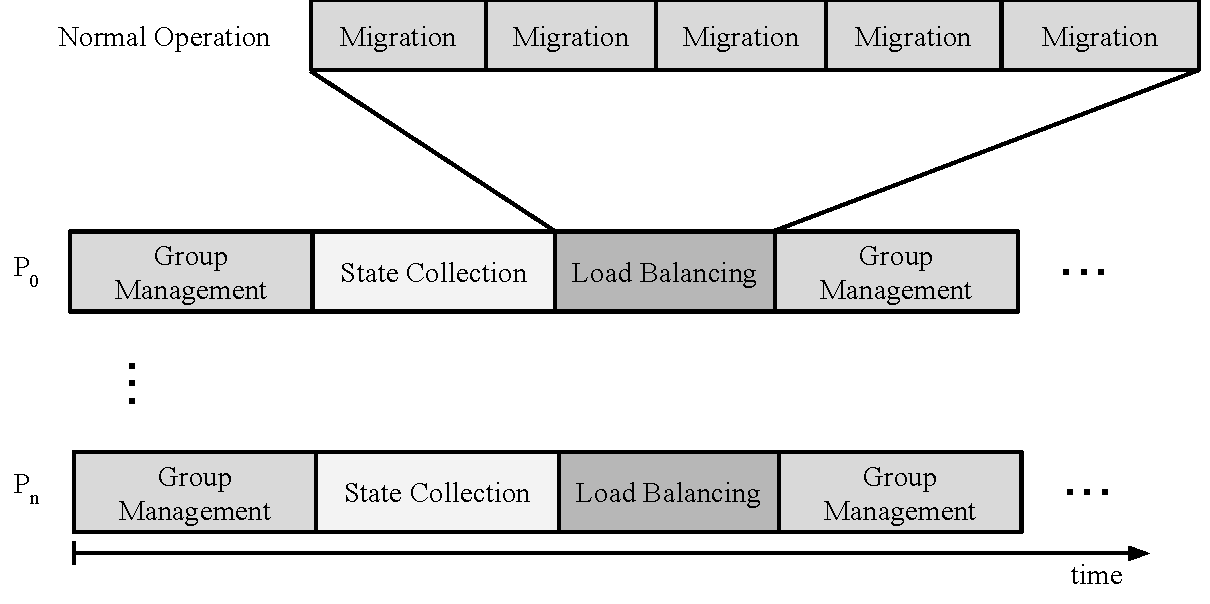
\includegraphics[width=0.85\linewidth]{NormalDGISchedule}
%\caption{Example of a \ac{DGI} schedule. During the execution of the Load Balancing module, work is performed to manage power devices.} \label{fig:normal-schedule}
%\end{figure}

\subsubsection{Leader Election.}

The \ac{DGI} uses a variation on the leader election algorithm, ``Invitation Election Algorithm,'' written by Garcia-Molina\cite{INVITATIONELECTION}.
This modified algorithm allows the interactions of the processes in our semi-synchronous system to be modeled with a Markov chain.
A version of this algorithm with a restriction on what processes could become coordinator is presented in \cite{JOURNAL}.
We elected to use an improved version of the algorithm in this work because of its easy-to-follow group state.

%This algorithm provides a robust election procedure which allows for transient partitions.
%Transient partitions are formed when a faulty link inside a group of processes causes the group to divide temporarily.
%These transient partitions merge when the link becomes more reliable.
The elected leader is responsible for making work assignments, identifying and merging with other coordinators when they are found, and maintaining an up-to-date list of peers.
Group members monitor the group leader by periodically checking if the group leader is still alive by sending a message.
If the leader fails to respond, the querying peers will enter a recovery state and operate alone until they can identify another coordinator.
Therefore, a leader and each of the members maintain a set of currently reachable processes, a subset of all known processes in the system.

Using a leader election algorithm allows the \ac{FREEDM} system to autonomously reconfigure rapidly in the event of a failure.
Cyber components are tightly coupled with the physical components, and reaction to faults is not limited to faults originating in the cyber domain.
Processes automatically react to crash-stop failures, network issues, and power system faults.
The automatic reconfiguration allows processes to react immediately to issues, faster than a human operator, without relying on a central configuration point.
However, it is important the configuration a leader election supplies is one where the system can do viable work without causing physical faults like voltage collapse or blackouts\cite{HARINI}.

%A state machine for the election portion of the election algorithm is shown in Figure \ref{fig:statemachine}.
%In the normal state, the election algorithm regularly searches for other coordinators to join with.
%When another coordinator is identified, all other processes will yield to their future coordinator.
%The method of selecting which process becomes the coordinator of the new group differentiates the modified algorithm from other approaches.

%Processes determine the optimal coordinator (the one with the lowest process ID) through the exchange of \ac{AYT} and \ac{AYC} messages.
%A process will only accept invites from processes more optimal than itself, and more optimal than its current leader.
%Once a timeout expires, the coordinator will send a ``Ready'' message with a list of peers to all processes that accepted the invite.
%To prevent live-lock the processes do not leave their previous group until the new Ready message arrives, unlike the original ``Invitation Election Algorithm.''
%The invited processes have timeouts for when they expect the ready message to arrive.
%
%Once a group is formed it must be maintained.
%To do this, processes occasionally exchange messages to verify the other is still reachable.
%%This interaction is shown in Figure \ref{fig:statemachine2}.
%Coordinators send \ac{AYC} messages to members of its group to check if the process has left the group.
%Group members send \ac{AYT} messages to the coordinator to verify they haven't been removed from the group, and to ensure the coordinator is still alive.
%If processes fail to reply to received message before a timeout, they will leave the group.
%Leaving the group can either be caused by the coordinator removing the process, or the process can enter a recovery state and leave the group, forming a new group by itself.

%This version also removes the potential live-lock due to crash failure, although crash-failure is not considered in this work.
%Other algorithms could be more efficient and less bursty during normal operation, however they are more inconsistent during network congestion and omission.

\subsubsection{Power Management.}

In this work we utilize the load balancing algorithm from \cite{LOADBALANCING}.
The load balancing algorithm performs work by managing power devices with a sequence of migrations\cite{HILTESTBED}.
In each migration, a sequence of message exchanges identify processes whose power devices are not sufficient to meet their local demand and other processes supply them with power by utilizing a shared bus.
%To do this, first processes that cannot meet their demand announce their need to all other processes.
%Processes with devices that exceed their demand offer their power to processes that announced their need.
%These processes perform a three-way handshake.
%At the end of the handshake, the two processes have issued commands to their attached devices to supply power from the shared bus and to draw power from the shared bus.

The \ac{DGI} algorithms can tolerate packet loss and is implemented using UDP to pass messages between \ac{DGI} processes.
Effects of packet loss on the \ac{DGI}'s group management module have been explored in \cite{CRITIS2012} and \cite{JOURNAL}.
The load balancing algorithm can tolerate some message loss, but lost messages can cause migrations to only partially complete, which can cause instability in the physical network.
%A failed migration is diagrammed in Figures \ref{fig:failed-migration-1} and \ref{fig:failed-migration-2}.
%With this power migration algorithm, uncompensated actions may occur in the power system.
These actions can eventually lead to power instability through issues such as voltage collapse.
%Additionally, the supply process may not always be certain if the second half of the action was completed or not.
%If the ``Draft Accept'' message does not arrive from the demand process, the supply process cannot be certain of whether or not its ``Draft Select'' message was received.
%If the supply process takes action to compensate by reversing the migration and the confirmation arrives later the system will also be driven towards instability because another process completed an uncompensated action.
%Processes could potentially confirm the number of failed migrations with a state collection technique.
%It is therefore desirable to manage the processes to minimize the number failed migrations.
In this work, we consider effects due to delays by congestion.

%\begin{figure}
%\centering
%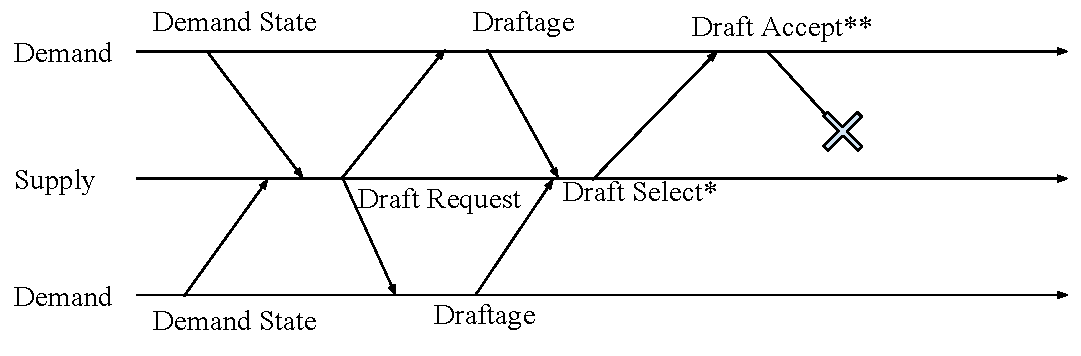
\includegraphics[width=0.95\textwidth]{FailedMigration1}
%\caption{Example of a failed migration. (*) and (**) mark moments when power devices change state to complete the physical component of the migration. In this scenario, the message confirming the demand side made the physical is lost, leaving the supply node uncertain.}
%\label{fig:failed-migration-1}
%\end{figure}
%
%\begin{figure}
%\centering
%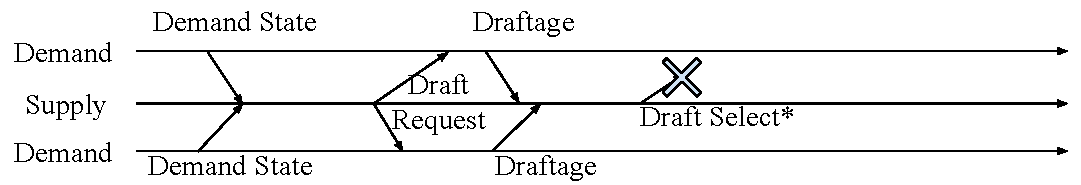
\includegraphics[width=0.95\textwidth]{FailedMigration2}
%\caption{Example of a failed migration. (*) marks a moment when power devices change state to complete the physical component of the migration. In this scenario, the supply process changes its device state, but the demand process does not.}
%\label{fig:failed-migration-2}
%\end{figure}

%A real-time system implementing this algorithm could count the number of failed migrations with a counter.
%The counter will increase when the physical side makes a change, increasing the number of outstanding migrations.
%The demand process will make their physical change and send the ``Draft Accept'' message.
%On receipt, the counter is reduced by one.
%A real-time deadline is enforced on the receipt of the ``Draft Accept'' -- if the message does not arrive before a specific time interval, the counter will not be decreased.

\subsection{Random Early Detection}
The \ac{RED} queueing algorithm is a popular queueing algorithm for switches and routers.
It uses a probabilistic model and an \ac{EWMA} to determine if the average queue size exceeds predefined values.
These values are used to identify potential congestion and manage it.
This is accomplished by determining the average size of the queue, and then probabilistically dropping packets to maintain the size of the queue.
In \ac{RED}, when the average queue size $avg$ exceeds a minimum threshold ($min_{th}$), but is less than a maximum threshold ($max_{th}$), new packets arriving at the queue may be ``marked''.
%The probability a packet is marked is based on the following relation between $p_{b}$ and $p_{a}$ where $p_{a}$ is the final probability a packet will be marked.

%\begin{equation}
%p_{b} = max_p (avg - min_{th}) / (max_{th}-min_{th})
%\end{equation}
%\begin{equation}
%p_{a} = p_{b} / (1-count * p_b)
%\end{equation}

%Where $max_p$ is the maximum probability a packet will be marked when the queue size is between $min_{th}$ and $max_{th}$ and $count$ is the number of packets since the last marked packet.
With \ac{RED}, the probability a packet is marked varies linearly with the average queue size, and as a function and the time since the last packet was marked.
If $avg$ is greater than $max_{th}$, the probability of marking trends toward 1 as the average queue size approaches $2*max_{th}$
In the event the queue fills completely, the \ac{RED} queue operates as a drop-tail queue.

In a simple implementation of the \ac{RED} algorithm, marked packets are dropped.
For a TCP application, the result of the dropped packets causes the slow-start congestion control strategy to reduce the rate packets are sent.
A more advanced implementation, using \ac{ECN}, sets specific bits in the TCP header to indicate congestion.
By using \ac{ECN}, TCP connections can reduce their transmission rate without re-transmitting packets.

UDP applications have not typically utilized \ac{ECN}.
Although the \ac{ECN} standard has flags in the IPv4 header, access to the IPv4 header is not possible on most systems.
Furthermore, there is not a ``one size fits all'' solution to congestion in UDP algorithms.
However, for the \ac{DGI} and a class of similar real-time processes, congestion notification has great potential.
If processes can adjust the amount of traffic they send based on the anticipated congestion (by disabling features, for example), they can decrease the effects of congestion.

\section{Experimental Setup}
\label{sect:experimentalsetup}

Experiments were run in a Network Simulator 3.23\cite{NS3} test environment.
The simulation time replaced the wall clock time in the \ac{DGI} for the purpose of triggering real-time events.
As a result, the computation time on the \ac{DGI}s for processing and preparing messages was neglected.
However, to compensate for the lack of processing time, the synchronization of the \ac{DGI}s was instead randomly distributed as a normal distribution.
This was done to introduce realism to ensure events did not occur simultaneously.
Additionally, the real-time schedules used by the \ac{DGI} were adjusted to remove the processing time that was neglected in the simulation.

The \ac{DGI}s were placed into a partitioned environment.
The test included 30 nodes.
Each of the nodes ran one \ac{DGI} process.
Two sets of 15 \ac{DGI} were each connect to a switch and each switch was in turn connected to the router.
This network is pictured in Figure \ref{fig:network-layout}.
Node identifiers were randomly assigned to nodes in the simulation and used as the process identifier for the \ac{DGI}.

The links between the router and the switches had a \ac{RED} enabled queue placed on both network interfaces.
The \ac{RED} parameters for all queues were set identically.
A summary of \ac{RED} parameters are listed in Table \ref{tab:red-parameters}.
All links in the simulation were 100Mbps links with a 0.5ms delay.
RED was used in packet count mode to determine congestion.
ARP tables were populated before the simulation began.
\ac{RED} parameters were selected using results from \cite{JOURNAL}.

%The relationship between the background traffic and the average queue size was estimated through runs of the \ac{NS3} simulation.
%Figure \ref{fig:plotm} demonstrates the observed relationship between the total background traffic and the maximum average queue size for that level of traffic.
%Additionally, the $DequeueRate$ was collected from a run of the simulation without traffic, and was found to be $713.08$ packets/second.
%Therefore, from Equation \ref{eq:prob-est}, assuming $init_q=0, resp=225, init_m=225$ and $\Delta t=1$, the maximum traffic rate with no omissions is $263.0$ packets/second.
%The number of packets for the $resp$ and $init_m$ were selected from the worst case of the algorithm in \cite{JOURNAL}.
%Based on the traffic parameters in Table \ref{tab:red-parameters}, $263.0$ packets/second corresponds to 1.077 Mbps of traffic generated at one switch and 2.1545 Mbps traffic overall.
%From the polynomial estimate in Figure \ref{fig:plotm}, the maximum average queue size for that level of traffic is $94.715$, estimated as $90$ for the \ac{RED} Min Threshold in Table \ref{tab:red-parameters}.
%RED Max Threshold is computed using a similar technique, but using the message complexity for the Load Balancing algorithm, since it maintains its complexity during Soft ECN mode.
%
%\begin{figure}
%\centering
%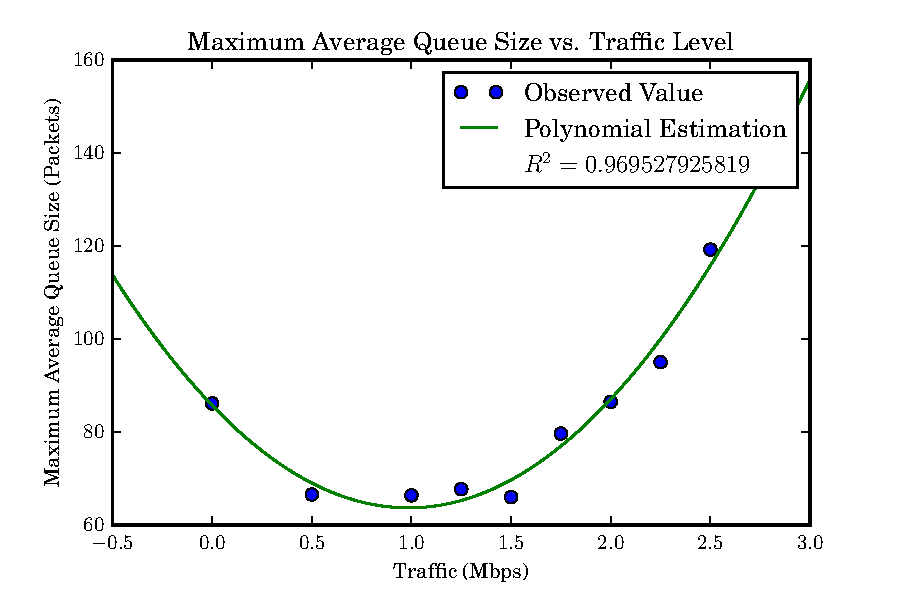
\includegraphics[width=0.65\linewidth]{m-max-average-queue.pdf}
%\caption{Plot of the maximum observed average queue size as a function of the overall background traffic. The polynomial estimate is $y=22.70x^2-44.74x+85.72$}
%\label{fig:plotm}
%\end{figure}

\begin{table}
\begin{center}
\begin{tabular}{ | l | l || l | l | } \hline
Parameter & Value & Parameter & Value        \\ \hline
RED Queueing Mode & Packet & RED Gentle Mode & True    \\ \hline
RED $Q_{w}$ & 0.002 & RED Wait Mode & True      \\ \hline
RED Min Threshold & 90 & RED Max Threshold & 130   \\ \hline
%Maximum Queue Size & 1000 \\ \hline
RED Link Speed & 100 Mbps & RED Link Delay & 0.5 ms   \\ \hline
%Clock Distribution $\sigma$ & 0.005 & Traffic Packet Size & 512 Bytes \\ \hline
\end{tabular}
\end{center}
\caption{Summary of \ac{RED} parameters. Unspecified values default to the \ac{NS3} implementation default value}
\label{tab:red-parameters}
\end{table}

To introduce traffic, processes attached to each of the switches attempted to send a high volume of messages to each other across the router.
The number of packets sent per second was a function of the data rate and the size of the packets sent.
In each simulation, half of the traffic originated from each switch.
Due to the bottleneck due to the properties of the network links, the greatest queueing effect occurred at the switches.
